\chapter{Приклади обчислень}
\begin{example}
Знайдіть ${\iint\limits_{D}\left(x^2+y^2\right)d x d y}$, де через $D$ позначений пря\-мо\-кут\-ник ${D = \segment{1}{2}\times\segment{2}{4}}$.

Спочатку зробимо рисунок області інтегрування $D$.

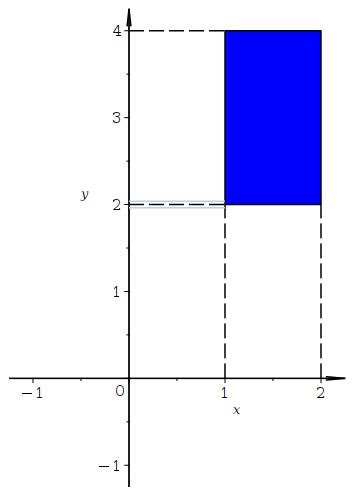
\includegraphics[width=0.25\paperwidth]{example.2.1}

Тепер застосуємо теорему про зведення кратного інтегралу до повторного:
\[
\iint\limits_{D}\left(x^2+y^2\right)d x d y = \int\limits_1^2\left(\int\limits_{2}^{4}\left(x^{2}+y^{2}\right)d y\right)dx.
\]
\begin{remark}
Можна було використати інший порядок змінних $x$ і $y$ і отримати
\[
\iint\limits_{D}\left(x^2+y^2\right)d x d y = \int\limits_{2}^{4}\left(\int\limits_1^2\left(x^{2}+y^{2}\right) d x\right)d y.
\]
В якості вправи пропонуємо підрахувати цей повторний інтеграл і переконатись, що відповідь буде така сама.
\end{remark}
Знайдемо спочатку $\int\limits_{2}^{4}\left(x^{2}+y^{2}\right)d y$. Нагадаємо властивість лінійності інтеграла Рімана:
\[
\int\limits_{a}^{b}\left(f(y)+g(y)\right)d y = \int\limits_{a}^{b}f(y)d y+\int\limits_{a}^{b}g(y)d y.
\]
Тут
\[
\begin{array}{cc}
f(y) = x^2 & \mbox{ --- не залежить від } y\mbox{, при інтегруванні вважається константою!}\\
g(y) = y^2 &
\end{array}
\]
\[
\int\limits_{2}^{4}\left(x^{2}+y^{2}\right)d y = \int\limits_{2}^{4}x^{2}d y+\int\limits_{2}^{4}y^{2}d y
\]

Для знаходження першого доданку ${\int\limits_{2}^{4}x^{2}d y}$ спочатку знайдемо первісну функції ${x^2}$ (яка не залежить від змінної $y$, тобто є в цьому інтегралі константою!):
\[
\int x^{2}d y = x^2 y + C,
\]
а потім скористаємось формулою Ньютона--Лейбніця:
\[
\int\limits_{2}^{4}x^{2}d y = x^2 y \biggr|_{y=2}^4 = 4 x^2 - 2 x^2 = 2 x^2.
\]
Для знаходження другого доданку ${\int\limits_{2}^{4}y^{2}d y}$ спочатку знайдемо первісну функції ${y^2}$:
\[
\int\limits_{2}^{4}y^{2}d y = \frac{y^3}{3} + C,
\]
а потім скористаємось формулою Ньютона--Лейбніця:
\[
\int\limits_{2}^{4}y^{2}d y = \frac{y^3}{3} \biggr|_{y=2}^4 = \frac{4^3}{3} - \frac{2^3}{3} = \frac{56}{3}.
\]
У підсумку,
\[
\int\limits_{2}^{4}\left(x^{2}+y^{2}\right)d y = \int\limits_{2}^{4}x^{2}d y+\int\limits_{2}^{4}y^{2}d y = 2 x^2 + \frac{56}{3}.
\]
Значить,
\[
\iint\limits_{D}\left(x^2+y^2\right)d x d y = \int\limits_1^2\left(\int\limits_{2}^{4}\left(x^{2}+y^{2}\right)d y\right)dx = \int\limits_1^2\left(2 x^2 + \frac{56}{3}\right)dx.
\]
Знайдемо останній інтеграл. Згідно з лінійністю інтеграла Рімана
\[
\int\limits_1^2\left(2 x^2 + \frac{56}{3}\right)dx = 2 \int\limits_1^2 x^2 d x + \frac{56}{3}\int\limits_1^2dx.
\]
Для знаходження першого доданку ${2\int\limits_1^2 x^2 d x}$ спочатку знайдемо первісну функції ${x^2}$ (тепер ми інтегруємо по змінній $x$, і тому ця функція не  є в цьому інтегралі константою):
\[
\int x^{2}d x = \frac{x^3}{3} + C,
\]
а потім скористаємось формулою Ньютона--Лейбніця:
\[
2\int\limits_{1}^{2}x^{2}d x = 2 \times\frac{x^3}{3} \biggr|_{1}^2 = 2\times \frac{2^3}{3} - 2\times \frac{1^3}{3} = \frac{14}{3}.
\]
Для знаходження другого доданку ${\frac{56}{3}\int\limits_1^2dx}$ спочатку знайдемо первісну константи ${1}$:
\[
\int\limits d x = x + C,
\]
а потім скористаємось формулою Ньютона--Лейбніця:
\[
\frac{56}{3}\int\limits_{1}^{2} d x = \frac{56}{3} x \biggr|_{1}^2 = \frac{56}{3}\times 2 - \frac{56}{3} \times 1 = \frac{56}{3}.
\]
У підсумку,
\[
\iint\limits_{D}\left(x^2+y^2\right)d x d y =  \int\limits_1^2\left(2 x^2 + \frac{56}{3}\right)dx = .\frac{14}{3} + \frac{56}{3} = \frac{70}{3}.
\]
Відповідь: ${\iint\limits_{D}\left(x^2+y^2\right)d x d y = .\frac{14}{3} + \frac{56}{3} = \frac{70}{3}.}$
\end{example}

\begin{example}
Знайдіть ${\iint\limits_{D}8 x^2 \sin\left(4 x y\right)d x d y}$, де через $D$ позначений пря\-мо\-кут\-ник ${D = \segment{\frac{\pi}{2}}{\pi}\times\segment{0}{1}}$.

Спочатку зробимо рисунок області інтегрування $D$.

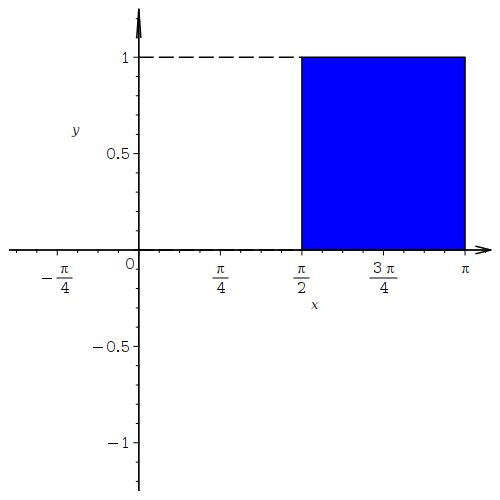
\includegraphics[width=0.25\paperwidth]{example.2.2}

Тепер застосуємо теорему про зведення кратного інтегралу до повторного:
\[
\iint\limits_{D}8 x^2 \sin(4 x y)d x d y = \int\limits_{\frac{\pi}{2}}^{\pi}\left(\int\limits_{0}^{1}8 x^2 \sin\left(4 x y\right)d y\right)dx.
\]

Знайдемо спочатку $\int\limits_{0}^{1}8 x^2 \sin\left(4 x y\right)d y$. Нагадаємо властивість лінійності інтеграла Рімана:
\[
\int\limits_{a}^{b}\alpha f(y) d y = \alpha \int\limits_{a}^{b}f(y)d y.
\]
Тут
\[
\begin{array}{cc}
f(y) =  \sin\left(4 x y\right) & \\
\alpha = 8 x^2  & \mbox{ --- не залежить від } y\mbox{, при інтегруванні вважається константою!}
\end{array}
\]
\[
\int\limits_{0}^{1}8 x^2 \sin\left(4 x y\right)d y = 8 x^2 \int\limits_{0}^{1} \sin\left(4 x y\right)d y.
\]
Тепер знайдемо первісну функції ${\sin\left(4 x y\right)}$:
\[
\int\limits \sin\left(4 x y\right)d y = -\frac{1}{4 x}\cos\left(4 x y\right) + C,
\]

а потім скористаємось формулою Ньютона--Лейбніця:
\[
\int\limits_{0}^1 \sin\left(4 x y\right)d y = -\frac{1}{4 x}\cos\left(4 x y\right) \biggr|_{y=0}^1 = -\frac{1}{4 x}\cos\left(4 x\right) - \left(-\frac{1}{4 x}\cos\left(0\right)\right) = \frac{1 - \cos \left(4 x\right)}{4 x}.
\]
У підсумку,
\[
\int\limits_{0}^{1}8 x^2 \sin\left(4 x y\right)d y = 8 x^2\times \frac{1 - \cos \left(4 x\right)}{4 x} = 2x \left(1 - \cos \left(4 x\right)\right).
\]
Значить,
\[
\iint\limits_{D}8 x^2 \sin(4 x y)d x d y = \int\limits_{\frac{\pi}{2}}^{\pi} 2x \left(1 - \cos \left(4 x\right)\right) d x.
\]
Знайдемо останній інтеграл. Для знаходження визначеного інтегралу
\[
\int\limits_{\frac{\pi}{2}}^{\pi} 2x \left(1 - \cos \left(4 x\right)\right) d x
\]
потрібно скористатись формулою інтегрування частинами:
\[
\int_a^b u d v = u v\biggr|_a^b - \int_a^b v d u.
\]
Тут
\[
\begin{array}{l}
u = 2 x, \\
d v = \left(1 - \cos \left(4 x\right)\right) d x.
\end{array}
\]
Для знаходження ${d u}$ потрібно продифференціювати (знайти похідну) ${u}$:
\[
d u  = \left(2 x \right)' d x = 2 d x,
\]
a для знаходження $v$ потрібно проінтегрувати ${d v}$:
\[
v = \int \left(1 - \cos \left(4 x\right)\right) d x \stackrel{{\normalfont\mbox{\tiny{(лінійність!})}}}{=} \int d x - \int \cos\left(4 x\right) d x = x - \frac{1}{4}\sin\left(4 x\right) + C.
\]
Таким чином,
\[
\begin{array}{l}
\int\limits_{\frac{\pi}{2}}^{\pi} 2x \left(1 - \cos \left(4 x\right)\right) d x = \left(2 x \left(x - \frac{1}{4}\sin\left(4 x\right)\right)\right)\biggr|_\frac{\pi}{2}^\pi - \int\limits_{\frac{\pi}{2}}^{\pi} \left(x - \frac{1}{4}\sin\left(4 x\right)\right) 2 d x = \\ =
\left(2 \pi \left(\pi - \frac{1}{4}\sin\left(4 \pi\right)\right)\right) - \left(2 \frac{\pi}{2} \left(\frac{\pi}{2} - \frac{1}{4}\sin\left(4\times \frac{\pi}{2}\right)\right)\right) - \int\limits_{\frac{\pi}{2}}^{\pi} \left(2x - \frac{1}{2}\sin\left(4 x\right)\right) d x = \\
=2\pi^2 - \frac{\pi^2}{2} - \int\limits_{\frac{\pi}{2}}^{\pi} \left(2x - \frac{1}{2}\sin\left(4 x\right)\right) d x = \frac{3\pi^2}{2} - \int\limits_{\frac{\pi}{2}}^{\pi} \left(2 x - \frac{1}{2}\sin\left(4 x\right)\right) d x.
\end{array}
\]
Для знаходження інтегралу ${\int\limits_{\frac{\pi}{2}}^{\pi} \left(2 x - \frac{1}{2}\sin\left(4 x\right)\right) d x}$ спочатку скористаємось лінійністю
\[
\int\limits_{\frac{\pi}{2}}^{\pi} \left(2 x - \frac{1}{2}\sin\left(4 x\right)\right) d x = 2\int\limits_{\frac{\pi}{2}}^{\pi} x d x - \frac{1}{2} \int\limits_{\frac{\pi}{2}}^{\pi} \sin\left(4 x\right) d x,
\]
потім знайдемо первісні функцій $x$ і $\sin\left(4 x\right)$
\[
\begin{array}{c}
\int x d x = \frac{x^2}{2} + C,\\
\int \sin\left(4 x\right) d x = -\frac{1}{4}\cos\left(4 x\right) + C,
\end{array}
\]
а потім скористаємось формулою Ньютона--Лейбніця:
\[
\begin{array}{c}
\int\limits_{\frac{\pi}{2}}^{\pi} x d x = \frac{x^2}{2}\biggr|_\frac{\pi}{2}^\pi = \frac{\pi^2}{2} - \frac{(\frac{\pi}{2})^2}{2} = \frac{\pi^2}{2} - \frac{\pi^2}{8} = \frac{3\pi^2}{8},\\
\int\limits_{\frac{\pi}{2}}^{\pi} \sin\left(4 x\right) d x = -\frac{1}{4}\cos\left(4 x\right)\biggr|_\frac{\pi}{2}^\pi = -\frac{1}{4}\cos\left(4 \pi\right) - \left(-\frac{1}{4}\cos\left(4 \times \frac{\pi}{2}\right)\right) = 0.
\end{array}
\]
У підсумку,
\[
\int\limits_{\frac{\pi}{2}}^{\pi} \left(2 x - \frac{1}{2}\sin\left(4 x\right)\right) d x = 2\int\limits_{\frac{\pi}{2}}^{\pi} x d x - \frac{1}{2} \int\limits_{\frac{\pi}{2}}^{\pi} \sin\left(4 x\right) d x = 2\times \frac{3\pi^2}{8} - \frac{1}{2} \times 0 = \frac{3\pi^2}{4},
\]
значить,
\[
\int\limits_{\frac{\pi}{2}}^{\pi} 2x \left(1 - \cos \left(4 x\right)\right) d x = \frac{3\pi^2}{2} - \frac{3\pi^2}{4} = \frac{3\pi^2}{4}.
\]
Остаточно,
\[
\iint\limits_{D}8 x^2 \sin(4 x y)d x d y = \frac{3\pi^2}{4}.
\]
Відповідь: ${\iint\limits_{D}8 x^2 \sin(4 x y)d x d y = \frac{3\pi^2}{4}.}$
\begin{remark}
В цьому прикладі ми також могли використати інший порядок змінних при зведенні до повторного інтегралу, і ми б отримали наступну рівність:
\[
\iint\limits_{D}8 x^2 \sin(4 x y)d x d y = \int\limits_{0}^{1}\left(\int\limits_{\frac{\pi}{2}}^{\pi}8 x^2 \sin\left(4 x y\right)d x\right)dy.
\]
Але в цьому випадку знаходження інтегралу всередині буде відносно складним і в результаті ми отримаємо
\[
\begin{array}{c}
\int\limits_{\frac{\pi}{2}}^{\pi}8 x^2 \sin\left(4 x y\right)d x = \\= -\dfrac{8 \pi^{2} y^{2} \cos \! \left(4 y \pi \right)-2 y^{2} \cos \! \left(2 y \pi \right) \pi^{2}-4 y \pi  \sin \! \left(4 y \pi \right)}{4 y^{3}}+\\
+\dfrac{2 y \sin \! \left(2 y \pi \right) \pi -\cos \! \left(4 y \pi \right)+\cos \! \left(2 y \pi \right)}{4 y^{3}}.
\end{array}
\]
Останній вираз потрібно буде ще проінтегрувати по $y$ від~$0$~до~$1$, що буде значно складніше наведеного розв'язання. Таким чином,

\fbox{
\begin{minipage}{0.7\textwidth}
\textbf{складність знаходження подвійного інтегралу може суттєво залежати від того, в якому порядку зводити його до повторного.}
\end{minipage}
}
\end{remark}
\end{example}
\begin{example}
Знайдіть ${\iiint\limits_{V}\left(x + y^2 - 2 z\right)d x d y d z}$, де через $V$ позначений пря\-мо\-кут\-ний паралелепіпед ${V = \segment{1}{2}\times\segment{1}{3}\times\segment{4}{5}}$.
Застосуємо теорему про зведення кратного інтегралу до повторного:
\[
\iiint\limits_{V}\left(x + y^2 - 2 z\right)d x d y d z = \int\limits_1^2\left(\int\limits_1^3\left(\int\limits_4^5\left(x + y^2 - 2 z\right)d z\right)d y\right)d x.
\]

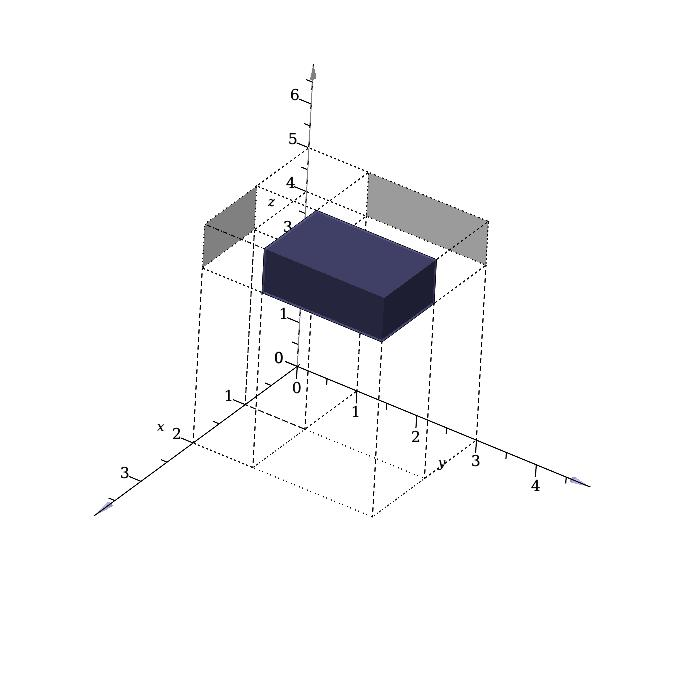
\includegraphics[width=0.5\paperwidth]{example.2.3}

Знайдемо спочатку ${\int\limits_4^5\left(x + y^2 - 2 z\right)d z}$. З лінійності інтеграла Рімана випливає, що
\[
\int\limits_4^5\left(x + y^2 - 2 z\right)d z = \int\limits_4^5xd z + \int\limits_4^5y^2d z - 2 \int\limits_4^5 zd z.
\]
Тепер знайдемо первісні відповідних функцій (пам'таємо, що інтегрування відбувається по змінній $z$, тому змінні $x$ та $y$ при цьому є константами):
\[
\begin{array}{c}
\int x d z = x z + C,\\
\int y^2 d z = y^2 z + C,\\
\int z d z = \frac{z^2}{2} + C,
\end{array}
\]

а потім скористаємось формулою Ньютона--Лейбніця:
\[
\begin{array}{c}
\int\limits_4^5 x d z = x z\biggr|_{z=4}^5 = 5 x - 4 x = x,\\
\int\limits_4^5 y^2 d z = y^2 z\biggr|_{z=4}^5 = 5 y^2 -4 y^2 = y^2,\\
\int\limits_4^5 z d z = \frac{z^2}{2}\biggr|_{z=4}^5 = \frac{25}{2} - \frac{16}{2} = \frac{9}{2},
\end{array}
\]
Таким чином,
\[
\int\limits_4^5\left(x + y^2 - 2 z\right)d z = x + y^2 - 2 \times .\frac{9}{2} = x + y^2 -9
\]
і
\[
\iiint\limits_{V}\left(x + y^2 - 2 z\right)d x d y d z = \int\limits_1^2\left(\int\limits_1^3\left(x + y^2 -9\right)d y\right)d x.
\]
Тепер шукаємо
\[
\int\limits_1^3\left(x + y^2 -9\right)d y \stackrel{{\normalfont\mbox{(лінійність)}}}{=} \int\limits_1^3 x d y  + \int\limits_1^3 y^2d y  - 9 \int\limits_1^3 d y.
\]
Тепер знайдемо первісні відповідних функцій (пам'таємо, що інтегрування відбувається по змінній $y$, тому змінна $x$ при цьому є константою):
\[
\begin{array}{c}
\int x d y = x y + C,\\
\int y^2 d y = \frac{y^3}{3} + C,\\
\int d y = y + C,
\end{array}
\]

а потім скористаємось формулою Ньютона--Лейбніця:
\[
\begin{array}{c}
\int\limits_1^3 x d y = x y\biggr|_{y=1}^3 = 3 x - x = 2 x,\\
\int\limits_1^3 y^2 d y = \frac{y^3}{3}\biggr|_{y=1}^3 = \frac{3^3}{3} - \frac{1^3}{3} = \frac{26}{3},\\
\int\limits_1^3 d y = y\biggr|_{y=1}^3 = 3 - 1 = 2.
\end{array}
\]
Далі
\[
\int\limits_1^3\left(x + y^2 -9\right)d y = 2 x  +\frac{26}{3} - 9 \times 2 = 2 x - \frac{28}{3}.
\]
і
\[
\iiint\limits_{V}\left(x + y^2 - 2 z\right)d x d y d z = \int\limits_1^2\left(2 x - \frac{28}{3}\right)d x.
\]
Знайдемо останній інтеграл.
\[
\int\limits_1^2\left(2 x - \frac{28}{3}\right)d x \stackrel{{\normalfont\mbox{(лінійність)}}}{=} 2 \int\limits_1^2 x d x - \frac{28}{3} \int\limits_1^2 d x.
\]
Первісні:
\[
\begin{array}{c}
\int x d x = \frac{x^2}{2} + c,\\
\int d x  = x + C.
\end{array}
\]
Тепер формула Ньютона--Лейбніця:
\[
\begin{array}{c}
\int x d x = \frac{x^2}{2}\biggr|_{1}^2 = \frac{2^2}{1} - \frac{1^2}{2} = \frac{3}{2},\\
\int d x  = x \biggr|_{1}^2 = 2 - 1 = 1,\\
\end{array}
\]
Остаточно,
\[
\iiint\limits_{V}\left(x + y^2 - 2 z\right)d x d y d z = 2 \times \frac{3}{2}- \frac{28}{3} \times 1 = -\frac{19}{3}.
\]
Відповідь: ${-\frac{19}{3}}$.
\end{example}
